\section{Resource Barriers: Power, Matter, and Availability}

A resource is matter in a usable condition. A periodic-table entry is not a supply chain. Silicon in rock is not a wafer, atmospheric nitrogen is not fertilizer, and a metal dispersed through discarded products is not a stock of qualified components.

Extraction, concentration, purification, transport, fabrication, and maintenance create availability. A technical system builds its resource base as it uses it. This makes resources historically changeable without making their conditions optional.

\subsection{Power and the Rate of Change}

\subhead{Energy needs an appointment}

An energy total says little about whether a task can be done here, now, at the required rate. A process needs a form of energy it can use, delivered at a location, through equipment, within a time window. A reservoir of fuel, a charged battery, a live electrical connection, and heat at a low temperature provide different capabilities.

Kardashev's civilization types made controllable power a way of imagining technological scale.\cite{kardashev1964transmission} A commonly used continuous interpolation is

\begin{equation}
K=\frac{\log_{10}P-6}{10},
\label{eq:kardashev}
\end{equation}

with $P$ in watts. A rise of one unit corresponds to ten orders of magnitude in power; a rise of 0.1 corresponds to one. The logarithm keeps an enormous range on one axis. It says little about what is done with the power.

The chemical and nuclear energy scales differ greatly. Chemical reactions rearrange electrons; fission and fusion alter nuclei. Nuclear electricity, hydropower, wind, and solar already show why civilization's power cannot be described as a single chemical-bond ceiling.\cite{jaffe2018physics,smil2017energy} Converting a source into controlled, affordable output introduces equipment, supply, waste, and operating constraints.

Deuterium-tritium fusion releases about 17.6~MeV per reaction. Making useful power from it requires a favorable balance among heating, reaction output, confinement, material survival, and the rest of the plant.\cite{atzeni2004physics} High energy per event is a starting condition for an engineering program, not a deployed power station.

\subhead{A rocket's account}

Chemical propulsion supplies a sharp example of an energy route imposing a mass penalty:

\begin{equation}
\Delta v=v_e\ln\frac{m_0}{m_f},
\qquad
\frac{m_0}{m_f}=\exp\left(\frac{\Delta v}{v_e}\right).
\end{equation}

$v_e$ is effective exhaust velocity, and $m_0/m_f$ the initial-to-final mass ratio. In this idealized relation, every additional $v_e$ of required velocity change multiplies the mass ratio by $e$. Real missions also encounter gravity and drag losses. Staging and other propulsion systems change the design problem; the exponential explains the severity of the chemical route's tradeoff.

The same lesson applies less dramatically to machines on Earth. A controller can know a desirable motion while the actuator lacks peak power or the energy store lacks endurance. Intelligence and available power are different entries in the account.

\subhead{Storage, computation, and the wrong comparison}

Battery specific energy and a fuel's heating value measure different parts of a working system. Electric and combustion drivetrains convert stored energy with different efficiencies; tanks, packs, motors, cooling, and operating conditions also matter.\cite{placke2017lithium,ziegler2021reexamining} Quoting the ratio of two storage figures is useful only after establishing what is being compared.

Computing limits such as those studied by Bremermann and Bekenstein operate under particular physical assumptions.\cite{bremermann1982minimum,bekenstein1981universal} They are not forecasts of near-term chip improvement. A very distant theoretical limit neither guarantees cheap progress toward it nor tells a robot how much power its joints require.

Four groups of conditions recur: a suitable material, an available energy supply, a controllable process, and a way to sustain the result. Material selection and thermodynamics make their interaction visible.\cite{callen1985thermodynamics,georgescu1971entropy} A powerful source without suitable equipment can be unusable; an elegant process without stable feedstock can be uneconomic.

\subsection{Borrowing Structures That Nature Already Built}

\subhead{The first inventory}

Wood arrives with a fibrous structure. Cotton arrives with useful cellulose. A river arrives with a flow and a drop in height. An animal arrives with metabolism, muscles, and control. Early technologies often began by selecting and arranging such structures rather than synthesizing their properties from simpler feedstocks.

This is an advantage supplied by history. Photosynthesis, evolution, and geology have already performed some of the work. The user still pays for access, processing, transport, and renewal.

As requirements grow, those inherited forms become insufficient. A natural fiber may not have the required strength; a naturally occurring material may not have the purity a device needs. The system begins to manufacture the condition it once found.

The resulting “ladder” has several axes: reaction barriers, purity, defect control, precision, equipment scale, and maintenance. Calling all of them activation energy would conceal the differences. A smaller chip can demand a larger control apparatus without its fabrication being described by one rising chemical barrier.

\subhead{From muscle to a constrained mechanism}

Mechanization separates parts of a task that a body supplies together. A cam or gear can restrict a mechanism to a repeatable motion. Water or another power source then drives it. The machine does not need to deliberate over every movement because some of the control has been built into geometry.

Textile machinery illustrates the change. A useful motion is extracted from skilled bodily coordination and organized into repeatable stages. Shafts, bearings, feedstock variation, wear, and adjustment still determine how repeatable it is. Mechanical constraint moves uncertainty into a different part of the process.

Water power also relocates production. It supplies sustained torque where a suitable flow and head can be used. Steam power later changed the geography of access to that torque. The transformation was a reorganization of energy, machinery, transport, and labor together.\cite{smil2017energy}

\subhead{Flows and accumulated stocks}

Solar-powered production depends on irradiance, collecting area, and conversion:

\begin{equation}
P=\Phi A\eta.
\end{equation}

$\Phi$ is radiation flux density in W/m$^2$, $A$ an area, and $\eta$ the conversion factor for the chosen boundary. The solar irradiance near Earth's orbit is about 1,361~W/m$^2$ at a surface normal to the rays, outside the atmosphere.\cite{prsa2016nominal} A landscape's annual average includes day, night, latitude, weather, and the actual process.

Biomass, food, fiber, and fodder compete for land, water, and ecological functions. Power density helps explain the spatial reach of an energy system.\cite{smil2015power} A stored fuel releases energy accumulated earlier; harvesting the current year's biomass depends on a current flow.

Fossil fuels allowed industry to draw heavily on accumulated stocks. This widened the available power flow and changed location, scale, and scheduling. It also created extraction, combustion, and environmental liabilities. The resource was useful because a technical system could connect the stock to machinery.

Trade can move the land and labor burdens of production across borders. Historical imports of cotton, timber, and food supported industrial concentration elsewhere. A local balance sheet can look lighter because part of its support has moved away.

\subsection{Breaking and Re-forming Bonds}

\subhead{Nitrogen as a resource}

The atmosphere contains abundant nitrogen. Agriculture needs it in chemically usable forms. The strength of the nitrogen molecule makes the conversion a kinetic challenge, while the full reaction has its own thermodynamic balance.\cite{erisman2008how,jia2014mechanistic}

The Arrhenius relation gives a common account of temperature sensitivity over an appropriate range:

\begin{equation}
k=A\exp\left(-\frac{E_a}{\mathcal RT}\right).
\label{eq:arrhenius}
\end{equation}

$k$ is a rate constant, $A$ its pre-exponential factor, $E_a$ an activation energy in J/mol, and $\mathcal R$ the gas constant. Changing $T$ can strongly change a rate. A catalyst changes the route and its effective barrier. The activation energy of that route is not simply the isolated nitrogen bond's dissociation energy.

Ammonia synthesis combines pressure, temperature, catalysis, feedstock preparation, separation, and heat management. Its hydrogen supply can dominate important parts of the energy and emissions account. Better catalysts and a different hydrogen route therefore change more than a control setting.

An AI system can help search catalysts, infer operating windows, diagnose a plant, or schedule power. Its contribution is measured through the changed process: less energy, higher yield, safer operation, less downtime, or another specified result.

Materials selection and lifecycle analysis follow this reasoning beyond the reactor.\cite{ashby2012materials,allwood2012sustainable} An excellent component can carry an expensive production history. A slightly less efficient component can sometimes outperform it over the full service life.


\begin{figure}[ht]
\centering
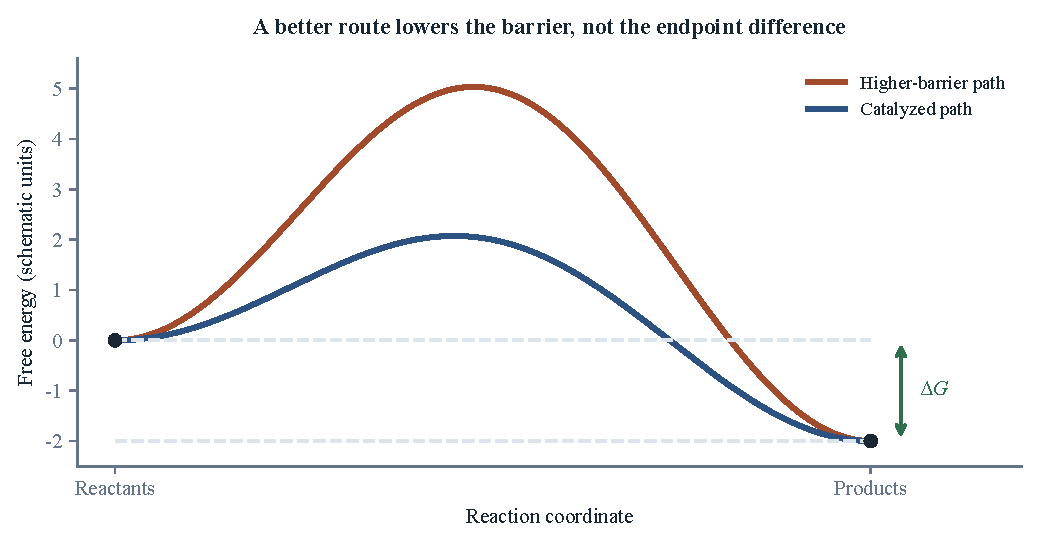
\includegraphics[width=\textwidth]{assets/activation-barrier.pdf}
\caption{A catalyst changes the route and its kinetic barrier. These schematic paths have identical endpoints and the same $\Delta G$. Lower activation free energy can accelerate reaction; the endpoint difference determines equilibrium.}
\label{fig:mechanism-activation-barrier}
\end{figure}
\subsection{The Weight of the Installed World}

\subhead{Past work made solid}

Cities contain accumulated extraction, processing, transport, lifting, assembly, finance, rules, and use. Roads and pipes occupy space and connect to occupied buildings. Their durability makes them useful and makes replacement a transition problem.

Research on global material stocks traces the huge accumulation of buildings and infrastructure during industrialization.\cite{krausmann2017global} Work on sediment flows likewise shows how extensively human activity moves and redirects material.\cite{syvitski2005impact} These stocks are a physical history with current users attached.

The work required to raise a mass through height $h$ in an approximately constant gravitational field is

\begin{equation}
W=mgh.
\end{equation}

For unchanged $m$ and $h$, a better drawing does not change this gravitational-energy difference. It can change the mass required, the construction route, or losses along that route. Lifting energy is one component of a building's account, often much smaller than the energy embodied in producing its materials.

The latest annual industry accounts keep the scale visible: world cement output is measured in billions of tonnes, and crude steel in roughly two billion tonnes.\cite{usgs2026cement,worldsteel2026figures} The relevant numbers are production flows, with stated years, not the full installed stock.

Replacing a district requires keeping services running, accommodating ownership, moving materials, and organizing a new configuration. A design can improve the destination while leaving the transition unaffordable. The installed world resists through the relations attached to its mass.

\subsection{Small Structures, Large Backends}

\subhead{Miniaturization changes the problem}

At smaller scales, mass becomes easier to move while defects, surface behavior, noise, tunneling, and heat become harder to manage. Semiconductor fabrication exposes the exchange. The product becomes small; the environment required to make it can become enormous.

The end of easy voltage and frequency scaling shifted more performance gains toward parallelism, specialized hardware, architecture, and packaging. “Dark silicon” describes a power-constrained gap between the transistors that fit on a chip and those that can operate at full activity together.\cite{esmaeilzadeh2011dark} Three-dimensional integration and other designs create new opportunities along with thermal and interconnect demands.

Thin barriers permit tunneling. Very small structures also turn discrete events into variability. Under a Poisson counting model,

\begin{equation}
\sigma_N=\sqrt N,\qquad \frac{\sigma_N}{N}=\frac{1}{\sqrt N}.
\end{equation}

To halve relative counting noise, four times as many events are required. Lithography has more mechanisms than photon counting alone, but stochastic exposure and resist behavior matter to defect control.\cite{debisschop2018stochastic} A nominal pattern and a reliably manufacturable pattern are different achievements.

\subhead{Heat has to leave}

A one-dimensional conductive approximation is

\begin{equation}
q''=\frac{P}{A}=-k_{\mathrm{th}}\frac{dT}{dx}.
\end{equation}

Heat flux density $q''$ has units W/m$^2$; $k_{\mathrm{th}}$ is conductivity. The sign follows the direction of decreasing temperature. Packaging adds interfaces, geometry, convection, and other heat paths. There is no universal air-cooling threshold for every device.

A facility repeats the problem at another scale. Concentrated computing needs power delivery and heat rejection. Better utilization and cooling can reduce demand per task.\cite{masanet2020recalibrating} Growth in tasks can still raise aggregate demand. In 2026, the IEA's account follows the network, supply, and connection constraints that accompany that growth.\cite{iea2026powering}

\subsection{Abundance, Concentration, and Recycling}

\subhead{Nature's inventory has a geography}

Primordial nucleosynthesis produced mostly hydrogen and helium. Later stellar and other nuclear processes produced heavier elements; planetary differentiation and geology redistributed them.\cite{steigman2007primordial,alpher1948origin,rudnick2003composition} A technical system inherits that distribution.

Abundance and availability diverge through concentration, location, chemistry, refining, equipment, and organization. For a mass fraction $\theta$, recovering a target mass $m$ requires at least

\begin{equation}
M=\frac{m}{\theta}
\end{equation}

of feedstock at perfect recovery. With recovery fraction $r<1$, the requirement becomes $m/(r\theta)$. Processing, energy, waste, and water demands depend on the actual ore and route, rather than only this inverse relation.

Critical-mineral studies follow the resulting concentrations in mining, refining, and supply chains.\cite{iea2021criticalminerals} Substitution can reduce dependence on one element while adding demands elsewhere. The useful question is which usable state the replacement requires.

\subhead{A second route through matter}

Recycling begins from a different initial state. Scrap aluminum already contains reduced metal; an ore route must perform reduction. Reuse can preserve even more of a component's fabrication history.

Collection, sorting, separation, purification, and requalification still have costs. Mixed materials, contamination, dispersion, and degradation can make a nominally recoverable stock difficult to use. The comparison is between routes, including their collection systems and the quality demanded of the result.

Across the scales, three obstacles recur: large stocks bind space and users; tiny structures magnify control demands; dispersed materials demand concentration. Intelligence can improve routes through all three. A useful route must still bring matter into the condition in which the function can exist.
